\documentclass[11pt]{article}
\usepackage[margin=1in]{geometry}
\usepackage[T1]{fontenc}
\usepackage[utf8]{inputenc}
\usepackage{lmodern}
\usepackage{enumitem}
\usepackage{hyperref}
\usepackage{xcolor}
\usepackage{tikz}
\usepackage{graphicx}
\usepackage{amsmath}
\usetikzlibrary{arrows.meta,positioning}
\hypersetup{colorlinks=true,linkcolor=blue!50!black,urlcolor=blue!50!black}
\setlist{nosep}
\definecolor{claude}{HTML}{7A55CC}
\definecolor{jev}{HTML}{2E9E63}
\definecolor{code}{HTML}{3A7BC0}

\title{Two Speeds of Mind:\\ a System One / System Two architecture for autonomous science}
\author{Kevin Horton}
\date{September 2026 \\ \small A vision paper; companion to the Jezero Ops demonstration}

\begin{document}
\maketitle

\begin{abstract}
Autonomous systems that must both \emph{act in real time} and \emph{reason about what to do} have historically been built from one of two poor choices: a single large model asked to do everything, or a pile of hand-tuned heuristics asked to be intelligent. We argue for a third shape, drawn from the way flight operations already divide labour between onboard software and a ground team, and from the dual-process picture of cognition: a \textbf{System Two} (a large language model) that plans, interprets, and argues from evidence at the cadence of a mission; a \textbf{System One} (a fast, calibrated, typed-judgment model) that answers narrow questions at the cadence of a control loop; and \textbf{code} that owns every rule, threshold, and unit of arithmetic in between. We built this on a Mars-rover simulation using real terrain and a real rover model, and found that the discipline it imposes --- \emph{numbers become words before a judgment is asked for; judgments become probabilities before a rule is applied; rules, not models, decide what happens next} --- is not a limitation but the source of the system's legibility and safety. We sketch the theory, the failure modes it avoids, and the research it invites.
\end{abstract}

\section{The problem: two cadences, one mind}

A rover on Mars lives at two speeds at once. Every few metres it must decide whether the dark shape ahead is a rock or a shadow, whether a bright patch will swallow a wheel, whether a telemetry blip means stop. Every sol it must decide what science is worth the energy, what the last sol's spectra mean for the hypotheses, whether a new request from a human is worth displacing the plan. The first kind of decision is \emph{closed}: the answer is one of a handful of options, it must be fast, and it must come with an honest estimate of its own uncertainty because a rule is going to act on it. The second kind is \emph{open}: it needs the whole context, it needs language, and it is allowed to take a minute and cost a dollar.

Large language models are extraordinary at the second kind and structurally wrong for the first. They are slow; they are expensive per call; and, decisively, they do not produce calibrated probabilities over a defined option set --- they produce text, from which a probability must be coaxed and cannot be trusted. Conversely, a fast typed-judgment model --- TypeSafe's \emph{jev} is the instance we used --- is built for the first kind and cannot do the second at all: it does not generate, reason in steps, or hold a plan.

The temptation is to pick one and stretch it. We think the right move is to keep both and make the boundary between them explicit, visible, and owned by code.

\section{The architecture}

Three engines, each trusted with exactly what it is good at.

\paragraph{System Two (LLM).} Given everything --- downlink, targets, hypotheses, history, and at science stops the actual camera frame --- it produces a \emph{structured} artefact against a schema: a sol plan with rationale, an interpretation with a lithology call and a next action, an assessment of a human's objective, a report. It also produces the one thing a System One cannot: \textbf{criteria in language} (``prioritise targets whose tone, texture, or fracture pattern differs visibly from the dark vesicular M\'aaz basalt\ldots'') that the System One will apply hundreds of times without further ground contact.

\paragraph{System One (typed judgment).} Given a \emph{filtered} state and a set of narrow questions --- a Choice over defined options, a yes/no Noul, a Score on ordered levels --- it returns a probability distribution per question in one call of a few hundred milliseconds, with a confidence derived from that distribution. It never sees the whole state; it never sees raw numbers it would have to reason over; it is never asked ``what should happen next?''

\paragraph{Code.} Perception geometry, budgets, ordering rules, thresholds, margins, the state machine, and --- most importantly --- the \emph{routing} decision: when to ask which model, and what to do when a model is unsure.

The information flow that results has a characteristic grammar:
\begin{center}
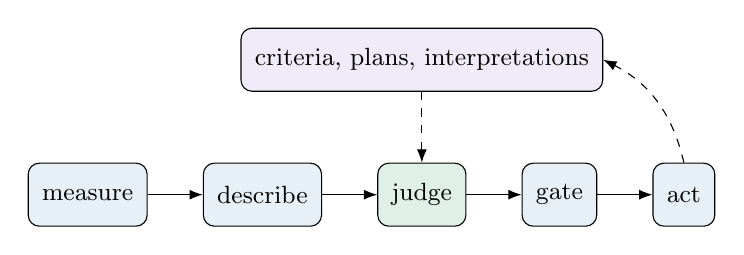
\begin{tikzpicture}[node distance=7mm, every node/.style={font=\small}, b/.style={draw, rounded corners, minimum height=8mm, inner sep=5pt}]
\node[b, fill=code!12] (m) {measure};
\node[b, fill=code!12, right=of m] (d) {describe};
\node[b, fill=jev!15, right=of d] (j) {judge};
\node[b, fill=code!12, right=of j] (g) {gate};
\node[b, fill=code!12, right=of g] (a) {act};
\node[b, fill=claude!12, above=9mm of j] (c) {criteria, plans, interpretations};
\draw[-{Latex}] (m) -- (d); \draw[-{Latex}] (d) -- (j); \draw[-{Latex}] (j) -- (g); \draw[-{Latex}] (g) -- (a);
\draw[-{Latex}, dashed] (c) -- (j); \draw[-{Latex}, dashed] (a.north) to[bend right=25] (c.east);
\end{tikzpicture}
\end{center}
Perception \emph{measures} (relief, extent, distance, tone). Code \emph{describes} those measurements in words the judgment model reads well (``knee-height, angular, mostly in shadow, stereo sparse''). The System One \emph{judges} ($P(\text{wheel hazard}) = 0.87$). Code \emph{gates} ($0.87 > 0.5 \Rightarrow$ obstacle; confidence $0.41 < 0.55 \Rightarrow$ do not act, re-image). Code \emph{acts} (ENav's nine arcs, with the new obstacle). The System Two enters this loop only at its edges: it wrote the criteria the judgments serve, and it reads the outcomes at the next downlink.


\begin{figure}[p]
\centering
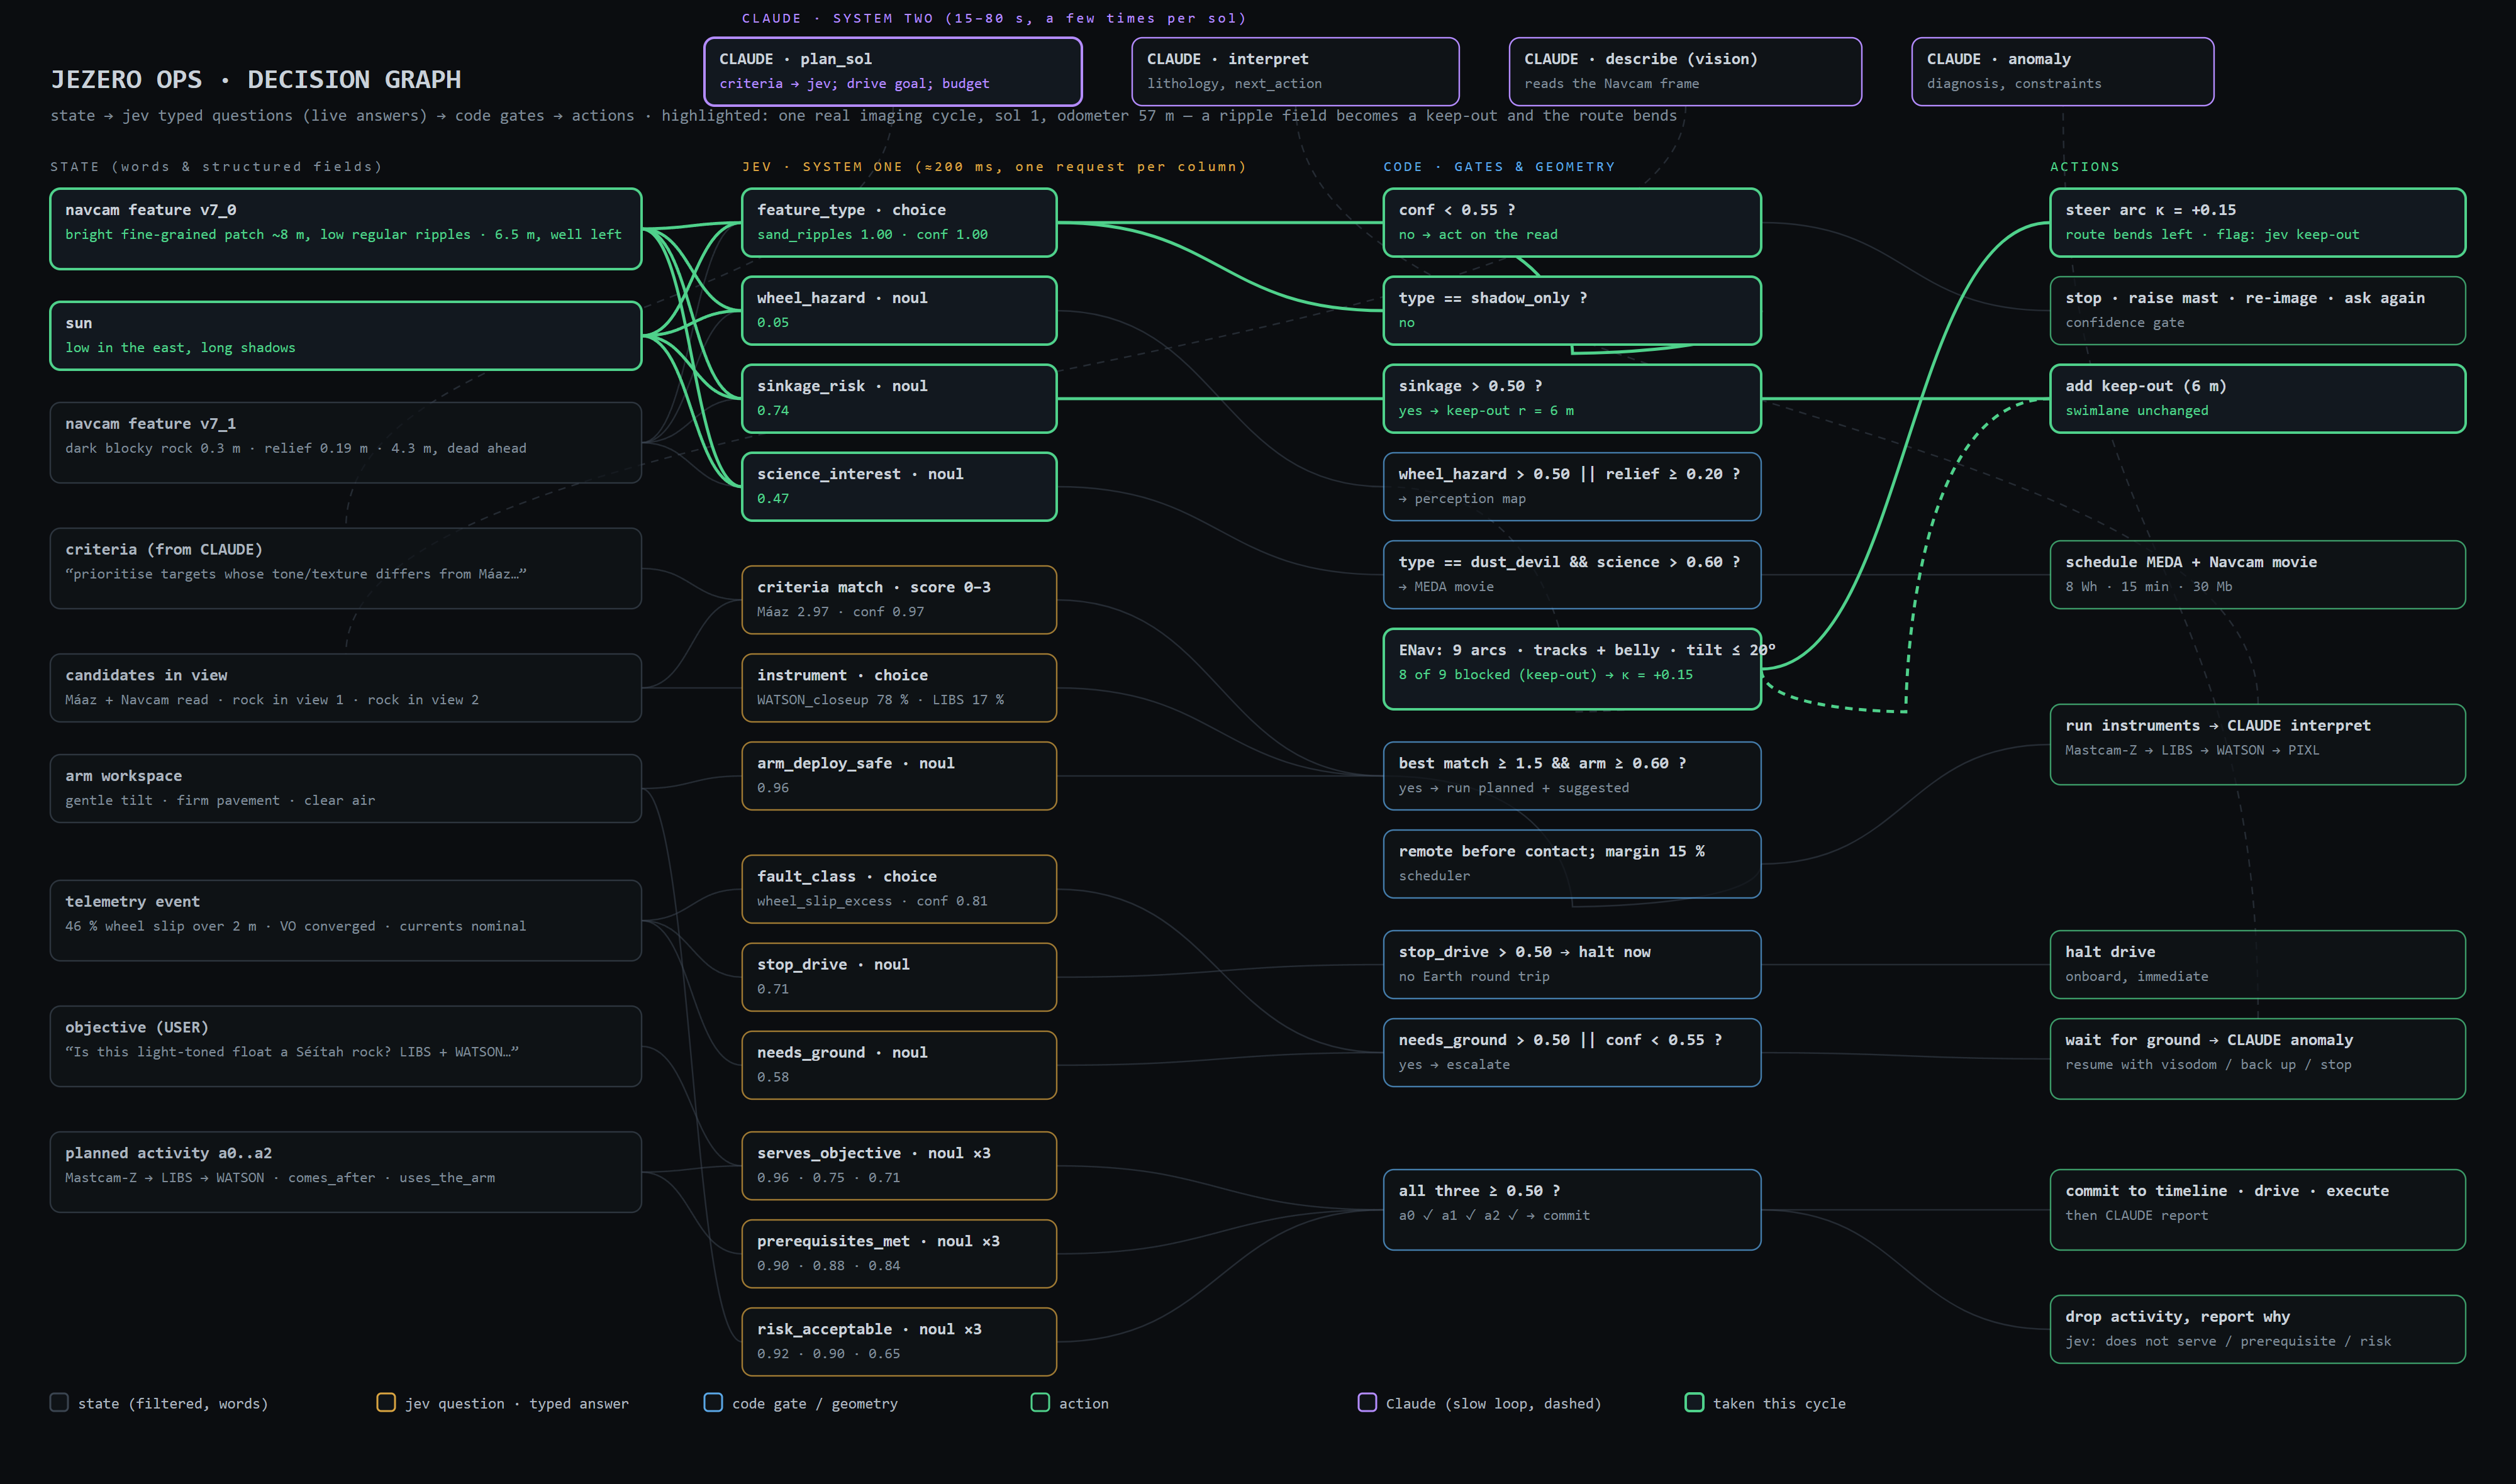
\includegraphics[width=\textwidth]{decision-graph.png}
\caption{The rover's decision graph in the style of TypeSafe's own demos. Left: the filtered state jev is shown (words, not raw numbers). Middle: jev's typed questions with their live answers --- a Choice returns an option and a confidence, a Noul a probability, a Score a position on ordered levels. Then the code gates that turn those numbers into actions, and the actions themselves. Claude's slow loop runs across the top and touches the graph only at its edges: it writes the criteria the middle column applies, and it reads the results. The lit path is a real cycle from the recorded run: a bright ripple field $\rightarrow$ \texttt{sand\_ripples} 1.00 / \texttt{sinkage\_risk} 0.74 $\rightarrow$ keep-out 6\,m $\rightarrow$ ENav finds 8 of 9 arcs blocked and steers $\kappa=+0.15$.}
\label{fig:graph}
\end{figure}

\section{Why the boundary is a feature}
Figure~\ref{fig:graph} shows the whole decision graph with one real cycle lit.


\paragraph{Calibration is the currency.} A rule can only be as good as the number it thresholds. A System One trained for calibrated decisions gives code something it can reason about: $0.87$ and $0.52$ are different, and a flat distribution across options is a signal in its own right. We used that signal directly --- a \emph{confidence gate} below which code refuses to act and instead buys more evidence (stop, raise the mast, image again). An LLM's ``I think it's probably a rock'' cannot be gated this way, and pretending otherwise is where systems get hurt.

\paragraph{Legibility is a by-product, not a feature to add.} Because every model call is a closed question with a typed answer, and every action is a rule over those answers, the system can show --- for every single decision --- which engine made it, what it was given, and what it returned. In the demonstration this is literally a colour: \textcolor{claude}{purple} for the LLM, \textcolor{jev}{green} for the judgment model, \textcolor{code}{blue} for code. An audit trail fell out of the architecture; it did not have to be designed.

\paragraph{The models can be swapped; the rules stay.} The thresholds (step limit, sinkage probability, confidence floor, scheduler margin) live in a policy file. The question sets are data. If a better judgment model appears, the rules do not change; if the LLM improves, the schemas do not change. The intelligence is replaceable; the discipline is the product.

\paragraph{Escalation is explicit.} Onboard halts are a rule over one number and need no Earth round trip ($P(\text{stop}) > 0.5$). Ground escalation is a second, separate number ($P(\text{needs ground})$), so the slow path is invoked only when the fast path \emph{says} it is out of its depth. This is exactly the shape of a flight-rule / anomaly-team split, expressed in probabilities.


\section{Where the boundary runs: through the chain of thought}
The obvious reading of the architecture is spatial: System Two on the ground, System One on the rover, code in between. The demonstration's last pass tested a stronger claim --- that the boundary can run \emph{through} the LLM's own reasoning without dissolving. We gave the planner the judge as a tool: while Claude writes a sol plan it can put typed questions to jev and get calibrated probabilities back in $\sim$300\,ms, and the prompts tell it what a planner does with such a tool (score candidates against the draft criteria, check an order against the rules, break ties, audit its own conclusion). Measured on the recorded run, 13 of 18 Claude calls consulted jev --- 13 consultations, 33 questions --- against 96 onboard calls; about 12\,\% of System One's work happened inside System Two's reasoning, at no meaningful cost in time (Figure~\ref{fig:graph2}).

What matters is what did \emph{not} change. jev still cannot reason, so Claude still decides what to ask and what the answer means. Claude still cannot calibrate itself, so when it asked whether its own WATSON run had been justified by its own rule, it got 0.05 and reported that. Code still records every consultation, still routes nothing to the rover except through Claude's schema, and still verifies that schema with the onboard jev afterwards. The two minds interleave at the granularity of a question; they do not merge.

\begin{figure}[p]
\centering
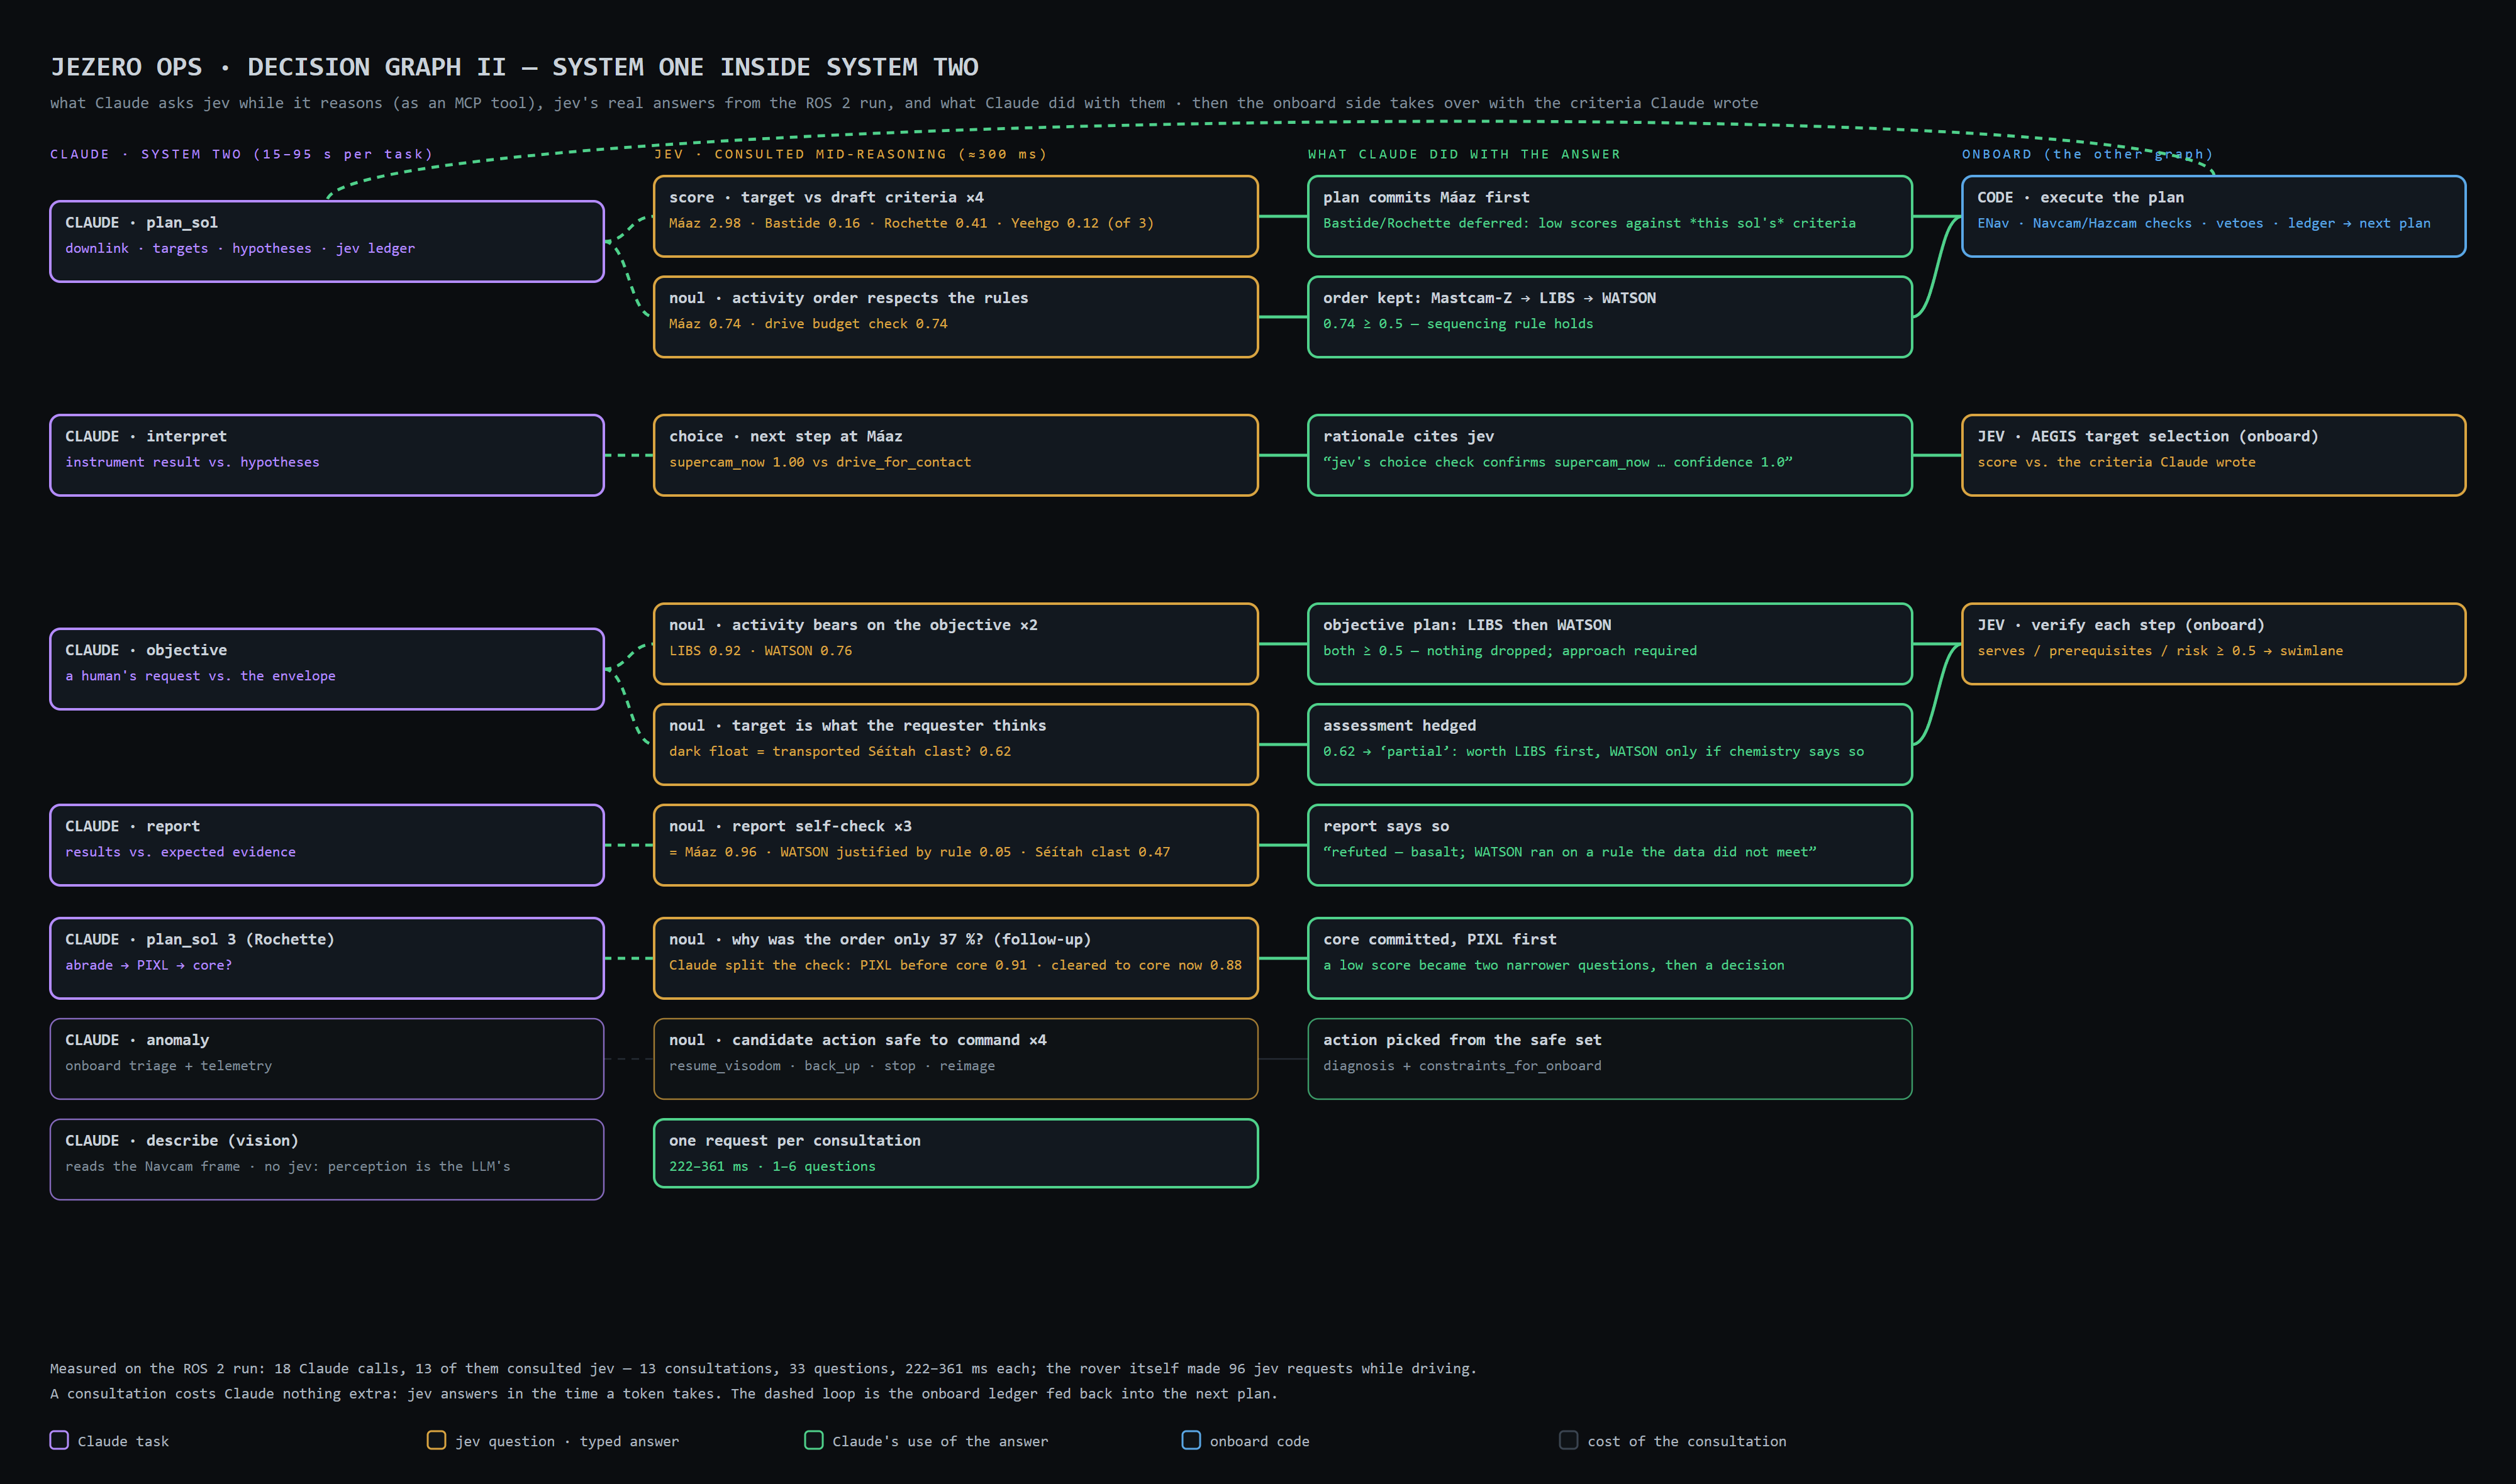
\includegraphics[width=\textwidth]{decision-graph-2.png}
\caption{Decision graph II: Claude's reasoning tasks, the typed questions each put to jev, jev's real answers, and what Claude did with them --- including asking why a score was low and splitting the question in two.}
\label{fig:graph2}
\end{figure}

\section{What we learned building it}

\begin{enumerate}
\item \textbf{``Perception'' that reads the world's truth table is not perception.} Our first driving loop looked up nearby rocks from the simulator's list. It worked and taught nothing. Replacing it with a rendered camera, a depth buffer as stereo, blob measurement, and deliberate dropout in shadow changed the character of every downstream judgment: shadows became a real question; rocks below the stereo threshold became a real hazard the rover could park on; the confidence gate started firing for honest reasons.
\item \textbf{Words are the right interface to a judgment model.} jev is text-only by design and weak at arithmetic; that is not a bug to route around but a reminder of where code belongs. Every quantity we tried to pass as a number worked better as a bucket (``shin-height'', ``a few metres ahead'', ``mostly in shadow''). The LLM, meanwhile, \emph{wants} the image --- and reading the actual Navcam frame produced field-geologist descriptions that were then handed, as words, to the System One for target selection. Vision belongs to System Two; judgment about what the vision found belongs to System One.
\item \textbf{Rules must be allowed to override their own inputs.} A rock inside the rover's footprint must not veto the move that gets the rover off it. A drive cap that would strand the rover metres short of its own goal is a planning slip, not intent. These guard rails only code can hold, and each one we added made the model calls \emph{more} useful, not less.
\item \textbf{Build it as a web page first, then move it to ROS\,2.} The prototype was HTML, CSS and three.js with a Node server holding the two model calls; every decision path was designed there. Moving it to ROS\,2 Jazzy took an afternoon precisely because the boundaries were already messages: the browser kept only what a simulator owns, and perception, judgment, ENav, the planner and the executive became five nodes with typed interfaces (Figure~\ref{fig:rosgraph}). Nothing about the rules or the questions changed --- only where they live, and the fact that a bag now replays every attributed decision.
\item \textbf{Humans inject objectives; the same machinery verifies them.} A person clicks a rock and states what they want. The LLM plans it inside the remaining budget; the System One verifies \emph{each planned step} (serves the objective? prerequisites met? risk acceptable now?) with probabilities before code commits resources; the LLM reports. The human's intent flows through the same measure--describe--judge--gate--act grammar as everything else, and is therefore just as auditable.
\end{enumerate}

\begin{figure}[t]
\centering
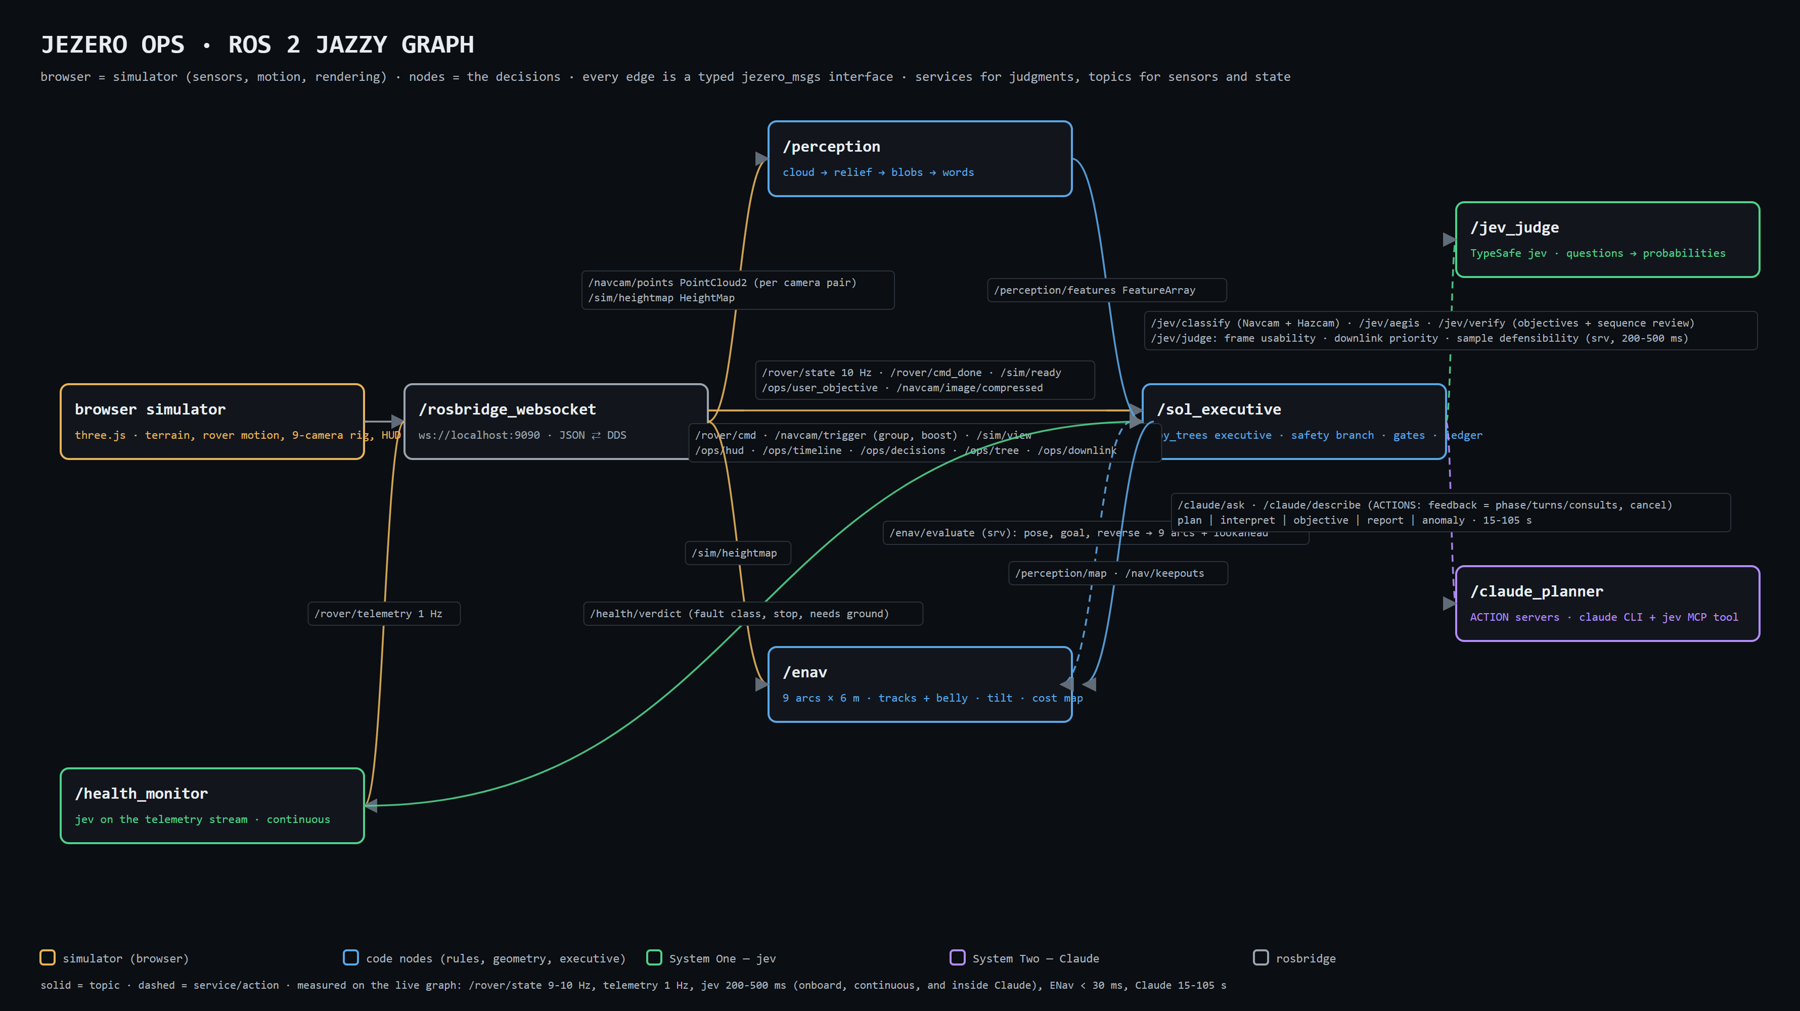
\includegraphics[width=\textwidth]{figs/ros2-graph.png}
\caption{The graph after the move to ROS\,2: gold the browser simulator, blue the code nodes, green jev behind four services, purple Claude behind two. Solid edges are topics, dashed are services.}
\label{fig:rosgraph}
\end{figure}

\section{Failure modes the architecture avoids}
\begin{itemize}
\item \textbf{The confident hallucination.} The LLM is never the last word on a safety-relevant fact; a typed judgment with a probability is, and code decides what probability is enough.
\item \textbf{The tuned-heuristic thicket.} The rules are few and legible because the semantic work is done by models; ENav is a hundred lines, not a thousand.
\item \textbf{The invisible decision.} Nothing happens without an attributed message; ``why did it turn left at 48\,m?'' has an answer in the log.
\item \textbf{The slow loop in the fast seat.} The LLM's 15--80\,s latency is a relay pass, not a control loop; the architecture makes that physically true by giving it no role in the drive cycle.
\end{itemize}

\section{Research directions}
\begin{itemize}
\item \textbf{The rover's judge, on every stream.} In the final build jev reads the housekeeping telemetry continuously, reviews the plan before uplink, gates each camera frame, scores where the arm should put its instrument and clears the contact from the hover, checks sample defensibility and orders the downlink --- fourteen closed questions on fourteen streams, none of them ``what should I do?'' The pattern held everywhere we tried it: measure, describe in words, ask a typed question, threshold, act, cite the rule. The open question is coverage: which of a rover's decisions \emph{cannot} be made this shape, and whether that set is empty.
\item \textbf{The planner's tool.} Giving System Two the judge as a tool worked on the first try and changed the plans it wrote. The open questions are about discipline: how many consultations are enough, whether the LLM can be trusted to phrase closed questions well (it can be prompted to; it can also be audited by a second judge), and whether a judge that sees the draft can be gamed by the draft. The recorded run shows one honest self-audit and one decomposition under doubt; that is evidence, not proof.
\item \textbf{Vision-native System One.} jev is text-only. A judgment model that could take the \emph{measured} feature crops (not raw frames) and return the same typed probabilities would collapse the describe step without giving up calibration. The question is whether calibration survives the modality change.
\item \textbf{Learning the gates.} Every threshold chosen by hand ($0.55$, $0.5$, $0.6$, $15\,\%$) is a candidate for learning against outcomes --- with the probabilities as features and the rules as the hypothesis class.
\item \textbf{Onboard deployment.} A System One at $\sim$200\,ms and a few hundred input tokens is within reach of rover-class compute in a way an LLM is not. The architecture already assumes the LLM is the ground segment; making that literal (Space ROS, a real relay-delay model) is a systems exercise --- and the first step is done: the graph runs as ROS\,2 Jazzy nodes, with the simulator on the other side of a rosbridge socket and every judgment a typed service call.
\item \textbf{Criteria as the contract.} The single most interesting artefact in the system is the sentence the LLM hands to the System One. It is a policy written in language, executed hundreds of times by a model that cannot write policy. How to test, version, and verify such contracts is an open problem with value well beyond rovers.
\item \textbf{Beyond rovers.} Any system with a slow deliberative loop and a fast reactive loop --- a surgical assistant, a trading desk, a warehouse --- has the same two cadences and the same temptation to collapse them.
\end{itemize}

\section{Conclusion}
We did not build a smarter rover. We built one whose intelligence is \emph{partitioned} --- a deliberative mind that plans and reads, a reactive mind that judges and is honest about its uncertainty, and a body of rules that decides which mind to ask and what to do with the answer. The partition is old; flight operations have used it for decades with humans in both roles. What is new is that both roles can now be filled by machines that are good at exactly one of them, and that the boundary between them can be drawn in code, in the open, one typed question at a time.

\vspace{1em}\noindent\small Demonstration, code and recorded run: \emph{Jezero Ops}, \texttt{C:\textbackslash Users\textbackslash Kevin\textbackslash Genai\textbackslash mars-rover-game}, and the Google Drive folder ``Jezero Ops --- Perseverance sim (Claude + jev)''.
\end{document}
